\chapter{Método de concatenación y selección de descriptores}\label{sec:metodo}

\section{Representación conjunta y pregunta de estudio}

El estudio evalúa la concatenación como un problema de selección de bloques. Cada extractor transforma una imagen $x_i$ en un vector $\mathbf{z}_{ij}\in\mathbb{R}^{d_j}$, donde $j$ identifica el descriptor y $d_j$ su dimensionalidad. Para un subconjunto $S$ de extractores, la representación conjunta se define como
\begin{equation}
 \mathbf{z}_{i,S}=\mathop{\Vert}_{j\in S}\frac{\mathbf{z}_{ij}}{\max(\lVert\mathbf{z}_{ij}\rVert_2,10^{-12})},
 \label{eq:concat}
\end{equation}
donde $\Vert$ denota concatenación. La normalización $L_2$ se aplica por descriptor y por muestra antes de unir los bloques, para evitar que la escala de un extractor determine por sí sola la contribución al clasificador.

La Figura~\ref{fig:pipeline} muestra cómo una misma imagen produce representaciones diferentes. Un descriptor resume patrones, relaciones entre intensidades o activaciones aprendidas en un vector. Después de normalizar cada bloque, se conserva un descriptor individual o se concatenan los bloques seleccionados. La dimensión conjunta es $d_S=\sum_{j\in S}d_j$.

\begin{figure}[!ht]
\centering
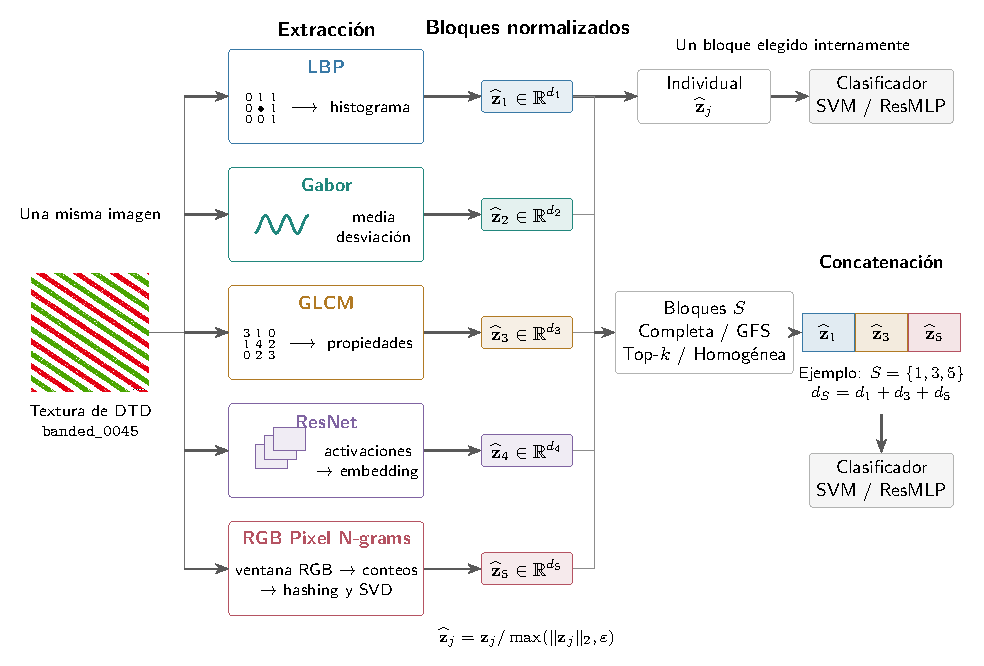
\includegraphics[width=\textwidth]{articulo/borrador_profesor/figures/concatenacion_v02.pdf}
\caption{Extracción y concatenación de descriptores. La misma imagen de DTD se representa mediante cinco ejemplos: patrones locales (LBP), respuestas de filtros (Gabor), coocurrencias (GLCM), una red convolucional (ResNet) y secuencias RGB (N-gramas). Las transformaciones internas se muestran esquemáticamente; no representan mapas de importancia por píxel. Cada rama produce un bloque normalizado que puede utilizarse individualmente o concatenarse con otros. El ejemplo de tres bloques ilustra la unión de coordenadas; cada política determina el subconjunto admisible.}
\label{fig:pipeline}
\end{figure}
\FloatBarrier

\section{Estrategias comparadas}

Las cinco estrategias responden a decisiones sobre la representación que recibe el clasificador. Individual establece el desempeño de un solo bloque; Completa evalúa la unión de toda la biblioteca; Top-$k$ y GFS eligen subconjuntos; Homogénea restringe la procedencia de los bloques a una familia. Se utilizan las mismas denominaciones en método, resultados y estadística:
\begin{enumerate}
\item \textbf{Individual}: descriptor con mayor macro-F1 medio en validación interna.
\item \textbf{Completa}: concatenación de todos los bloques de la biblioteca evaluada.
\item \textbf{Top-$k$}: concatenación de los $k$ descriptores mejor posicionados por su macro-F1 individual interno; $k$ se toma del subconjunto GFS de la misma condición.
\item \textbf{GFS}: subconjunto devuelto por la selección secuencial de bloques.
\item \textbf{Homogénea}: mejor resultado interno de GFS restringido a una familia, con un límite de bloques no mayor que el subconjunto GFS heterogéneo.
\end{enumerate}
Top-$k$ controla la composición bajo el mismo número de bloques que GFS, aunque las dimensiones pueden diferir. No constituye una política independiente de elección de $k$. Homogénea permite estudiar el efecto de restringir la biblioteca a una familia. Todos los comparadores se seleccionan antes de evaluar el test. Los controles aleatorios y las variantes de presupuesto se conservan como análisis auxiliares en los materiales del proyecto.

\section{Espacio de descriptores}

La biblioteca contiene 21 descriptores, agrupados según el tipo de representación. Cada uno constituye un bloque candidato sujeto al mismo criterio de selección. Las
Tablas~\ref{tab:extractores-clasicos} y~\ref{tab:extractores-aprendidos}
identifican la parametrización, los checkpoints y la dimensionalidad de cada
bloque. Las redes preentrenadas se ejecutaron en modo evaluación y sin
ajuste de pesos. En los modelos cargados mediante \texttt{timm} se eliminó la
capa clasificadora (\texttt{num\_classes=0}) y se aplicó el preprocesamiento
asociado al checkpoint. Para ViT, DeiT, Swin, MAE y SigLIP se utilizó la salida
\emph{pooler} cuando estaba disponible y, en caso contrario, el token de
clasificación. Todas las imágenes se convirtieron a RGB.

Los descriptores clásicos se basan en operadores LBP,
Gabor, GLCM y HOG \citep{ojala2002lbp,mehta2016drlbp,jain1991gabor,haralick1979glcm,dalal2005hog}.
Las CNN corresponden a VGG16, ResNet, DenseNet, EfficientNet y ConvNeXt V2
\citep{simonyan2015vgg,he2016resnet,huang2017densenet,tan2019efficientnet,woo2023convnextv2}.
El grupo Transformer incluye ViT, DeiT, Swin y EVA-02
\citep{dosovitskiy2021vit,touvron2021deit,liu2021swin,fang2024eva02}; las
representaciones con preentrenamiento autosupervisado o multimodal se basan en
DINOv2, MAE y SigLIP \citep{oquab2024dinov2,he2022mae,zhai2023siglip}.

\begin{table}[!ht]
\centering
\caption{Seis descriptores basados en patrones, filtros, gradientes y conteos incluidos en la biblioteca. Cada fila constituye un bloque completo.}
\label{tab:extractores-clasicos}
\fontsize{9}{11}\selectfont
\begin{tabular}{@{}lp{7.0cm}p{3.2cm}r@{}}
\toprule
Descriptor & Parametrización & Salida & Dim. \\
\midrule
LBP & multiescala $(P,R)=(8,1),(16,2),(24,3)$; mapeo uniforme invariante a rotación (riu2) & histogramas normalizados & 54 \\
LBP-rot & $P=8$, $R=1$; ocho rotaciones; códigos limitados a $[0,10]$ & histogramas $10\times 8$ & 80 \\
Gabor & cuatro frecuencias 0,1--0,8; seis orientaciones & media y desv. de respuesta real & 48 \\
GLCM & 256 niveles; distancias 1--3; cuatro ángulos; seis propiedades & promedios sobre ángulos & 18 \\
HOG & nueve orientaciones; celda $16^2$; bloque $2^2$; norma L2-Hys & vector HOG & 1.764 \\
N-gramas & ventana vertical $2\times1$; cuantización RGB por 12; 8.192 bins; SVD & vector normalizado & 256 \\
\bottomrule
\end{tabular}
\end{table}

\begin{table}[!ht]
\centering
\caption{Quince representaciones aprendidas congeladas incluidas en la biblioteca. ``Preclas.'' designa la salida inmediatamente anterior al clasificador del backbone.}
\label{tab:extractores-aprendidos}
\fontsize{9}{11}\selectfont
\begin{tabular}{@{}llp{6.5cm}lr@{}}
\toprule
Familia & Descriptor & Checkpoint & Salida & Dim. \\
\midrule
CNN & VGG16 & \texttt{vgg16.tv\_in1k} & preclas. & 4.096 \\
 & ResNet-50 & \texttt{resnet50.a1\_in1k} & preclas. & 2.048 \\
 & ResNet-101 & \texttt{resnet101.a1\_in1k} & preclas. & 2.048 \\
 & DenseNet-121 & \texttt{densenet121.tv\_in1k} & preclas. & 1.024 \\
 & EfficientNet-B0 & \texttt{efficientnet\_b0.ra\_in1k} & preclas. & 1.280 \\
 & ConvNeXt V2-T & \texttt{convnextv2\_tiny.fcmae\_ft\_in22k\_in1k} & preclas. & 768 \\
\midrule
Transformer & ViT-B/16 & \texttt{google/vit-base-patch16-224} & pooler/CLS & 768 \\
 & DeiT-S & \texttt{facebook/deit-small-patch16-224} & pooler/CLS & 384 \\
 & Swin-T & \texttt{microsoft/swin-tiny-patch4-window7-224} & pooler & 768 \\
 & EVA-02 base & \texttt{eva02\_base\_patch14\_224} & preclas. & 768 \\
\midrule
Autosup./multimodal & DINOv2-S & \texttt{vit\_small\_patch14\_dinov2.lvd142m} & preclas. & 384 \\
 & DINOv2-B & \texttt{vit\_base\_patch14\_dinov2.lvd142m} & preclas. & 768 \\
 & DINOv2-L & \texttt{vit\_large\_patch14\_dinov2.lvd142m} & preclas. & 1.024 \\
 & MAE-B & \texttt{facebook/vit-mae-base} & pooler/CLS & 768 \\
 & SigLIP-B & \texttt{google/siglip-base-patch16-224} & pooler/CLS & 768 \\
\bottomrule
\end{tabular}
\end{table}

Los descriptores clásicos se calcularon en escala de grises con la implementación de scikit-image: LBP, LBP-rot, Gabor y GLCM sobre imágenes redimensionadas a $256\times256$, y HOG sobre $128\times128$. LBP-rot designa la implementación propia registrada como \texttt{drlbp} en los archivos experimentales: aplica LBP con mapeo \texttt{ror} a ocho rotaciones y concatena diez bins por rotación en el intervalo $[0,10]$. Los códigos fuera de ese intervalo se descartan; por tanto, es un histograma restringido, no una reproducción del DRLBP de Mehta y Egiazarian \citep{mehta2016drlbp}. Los 21 vectores concatenados suman 19.884 dimensiones. Las características fijas y los conteos por imagen se almacenaron junto con etiquetas, orden de muestras y hashes de procedencia; las transformaciones aprendidas se ajustaron dentro de cada partición de entrenamiento. El estudio evalúa la selección y concatenación de bloques con extractores de imagen congelados y transformaciones ajustadas dentro del entrenamiento; no compara estrategias de \emph{fine-tuning}.

RGB Pixel N-grams \citep{paiva2023rgb} utiliza ventanas verticales de $2\times1$ píxeles con paso 1 sobre la imagen RGB en su resolución original. Cada canal se cuantiza mediante $q(v)=\lfloor v/12\rfloor$; los seis valores se codifican en base 22, recorriendo las dos posiciones de R, G y B. Los conteos se agrupan por el resto del código dividido por 8.192 y se comprimen mediante TruncatedSVD aleatorizado (256 componentes, cinco iteraciones y semilla de la condición). SVD se ajusta exclusivamente con el entrenamiento de cada partición interna y se reajusta sobre el entrenamiento externo para la evaluación final. El vector se normaliza con $L_2$ antes de concatenarlo. Esta parametrización comprimida se identifica como N-gramas + SVD y constituye una familia propia para la selección Homogénea.

\section{Greedy Forward Selection}

GFS se utiliza como un método \emph{wrapper}: los subconjuntos se valoran mediante el propio clasificador y exclusivamente dentro de la validación interna, como requieren los diseños de selección que separan búsqueda y evaluación externa \citep{kohavi1997wrappers,guyon2003feature}. La búsqueda comienza con un conjunto vacío. En el paso $t$, evalúa cada descriptor aún no seleccionado al añadirlo al subconjunto vigente y elige el candidato con mayor macro-F1 medio en la validación interna:
\begin{equation}
 j_t=\arg\max_{j\notin S_{t-1}}\widehat{F}_{1,\mathrm{inner}}(S_{t-1}\cup\{j\}),
 \qquad S_t=S_{t-1}\cup\{j_t\}.
 \label{eq:gfs}
\end{equation}
La búsqueda se limita a $k\leq 8$. Se detiene cuando la mejora respecto del paso anterior es menor que 0,001 durante dos pasos consecutivos, pero devuelve el mejor paso histórico, no necesariamente el último. Los empates se resuelven de forma determinista mediante el nombre del extractor. Todas las evaluaciones candidatas utilizan únicamente muestras pertenecientes al entrenamiento externo.

La Figura~\ref{fig:gfs-pasos} representa el mecanismo general de GFS. En cada ronda se comparan únicamente los bloques aún disponibles dentro de los folds internos; el bloque elegido se incorpora al subconjunto y el test externo permanece fuera de esa decisión.

\begin{figure}[!ht]
\centering
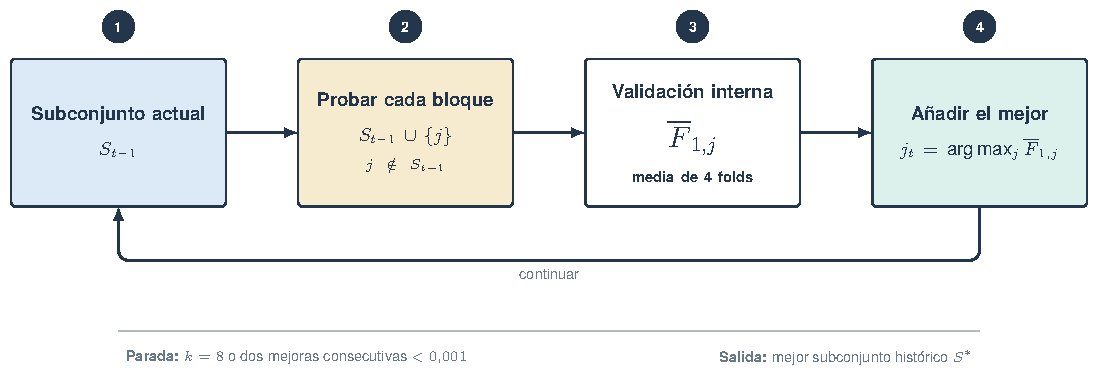
\includegraphics[width=\textwidth]{articulo/borrador_profesor/figures/gfs_pasos.pdf}
\caption{Mecanismo de Greedy Forward Selection sobre bloques completos. En cada paso se elige el bloque que maximiza el macro-F1 medio de la validación interna; el test externo se utiliza únicamente tras cerrar el subconjunto.}
\label{fig:gfs-pasos}
\end{figure}
\FloatBarrier

La Tabla~\ref{tab:config-gfs} concentra los parámetros de búsqueda, comunes a ambos clasificadores.

\begin{table}[!b]
\centering
\caption{Configuración de la selección GFS en el flujo general.}
\label{tab:config-gfs}
\fontsize{9}{11}\selectfont
\begin{tabular}{lp{8.4cm}}
\toprule
Elemento & Configuración \\
\midrule
Unidad de selección & Bloque completo generado por un extractor \\
Candidatos & 21 bloques \\
Criterio interno & Macro-F1 medio en cuatro folds estratificados y agrupados \\
Presupuesto & Hasta $k=8$ bloques \\
Parada & Dos mejoras consecutivas menores que 0,001; se devuelve el mejor paso histórico \\
Empates & Nombre del extractor, en orden determinista \\
Información excluida & Test externo y sus etiquetas durante toda la selección \\
\bottomrule
\end{tabular}
\end{table}
\FloatBarrier


\section{Conjuntos de datos y control de integridad}

Antes del análisis se construyó un manifiesto por dataset y se verificaron etiquetas, orden de muestras, dimensiones, valores finitos y grupos de dependencia. Se utilizaron DTD, FMD, CUReT y Outex. Sus particiones se describen a continuación; los cuatro datasets integran el análisis estadístico principal.

DTD contiene 5.640 imágenes de texturas en condiciones no controladas y proporciona diez particiones oficiales de entrenamiento, validación y prueba \citep{cimpoi2014dtd}. En cada partición se unieron entrenamiento y validación para ejecutar la selección interna, mientras que el test oficial se reservó para una única evaluación. Los duplicados byte-idénticos que cruzaban roles fueron retirados del conjunto de entrenamiento, conservando intacta la evaluación.

FMD reúne 1.000 fotografías de diez categorías de materiales \citep{sharan2013fmd}. Las características fijas y los conteos por imagen se obtuvieron desde las imágenes oficiales en un orden canónico. Cada imagen presentó un hash único y se utilizó como unidad de agrupación. La evaluación externa empleó cinco folds estratificados y agrupados, repetidos con semillas 42, 123 y 2026.

Outex contiene 1.360 BMP RGB de $128\times128$ píxeles, organizados en 68 clases balanceadas. La auditoría verificó archivos legibles, IDs continuos 000000--001359, ausencia de duplicados y la partición oficial de 680 imágenes de entrenamiento y 680 de prueba, con diez muestras de cada clase en cada lado \citep{ojala2002outex}. Todos los bloques respetan el orden de las 1.360 muestras del manifiesto oficial. Este es el único conjunto Outex utilizado en los resultados del artículo.

Para CUReT se utilizó la distribución gris recortada de 61 materiales, con 92 condiciones compartidas por clase \citep{varma2003filter}. Cada condición constituye un grupo para impedir que la misma configuración de adquisición aparezca a ambos lados de una partición. Se definieron dos mitades complementarias deterministas de 46 condiciones: A para selección y entrenamiento con B como test, y la dirección inversa. Esta asignación reproduce de manera transparente el tamaño 46/46 publicado, pero no se presenta como el split histórico exacto. Debido a que las dos direcciones son complementarias y dependientes, sus resultados se interpretarán descriptivamente.

\section{Clasificadores}

Se emplearon dos clasificadores con sesgos diferentes. La SVM lineal se implementa con \texttt{LinearSVC} de scikit-learn: $C=1$, ponderación balanceada por clase, pérdida \emph{squared hinge}, regularización $L_2$, esquema uno-contra-el-resto, tolerancia $10^{-4}$ y un máximo de 10.000 iteraciones.

Se denomina ResMLP a la MLP residual implementada para este estudio sobre vectores de características; no es una reproducción del modelo de imágenes del mismo nombre \citep{touvron2021resmlp}. Proyecta la entrada a 256 unidades y aplica tres bloques residuales, normalización de capa, activaciones GELU, \emph{dropout} de 0,1 y una salida multiclase. Se entrena con entropía cruzada y AdamW, tasa de aprendizaje $10^{-3}$, decaimiento de pesos $10^{-4}$, lotes de 256 muestras y un máximo de 100 épocas. La parada se basa en la pérdida media de entrenamiento: tras diez épocas sin una disminución mayor que $10^{-4}$, se detiene y restaura el mejor estado registrado. No utiliza el test ni una validación adicional para elegir la época. Las semillas se fijan para NumPy y PyTorch; cuando está disponible, la red se ejecuta en GPU.

\section{Configuración experimental y protocolo anidado}

La selección interna utiliza cuatro folds estratificados y agrupados. En DTD se ejecuta dentro de la unión \emph{train+val} de cada split oficial; en FMD dentro del entrenamiento de cada uno de los 15 folds externos; y en CUReT dentro de la mitad de 46 condiciones asignada al entrenamiento. En Outex, las cinco estrategias restringen los cuatro folds internos a las 680 imágenes del entrenamiento oficial. Después de seleccionar el subconjunto y los comparadores, cada modelo se ajusta con todo el entrenamiento externo y se evalúa una sola vez en el test correspondiente. Se verifica programáticamente que ningún grupo aparezca en entrenamiento y prueba.



\section{Análisis estadístico}\label{sec:analisis-estadistico}

El análisis utiliza rankings de Friedman y Quade, contrastes globales y comparaciones por pares con ajuste de Holm, siguiendo una organización empleada en clasificación de texturas \citep{paiva2023rgb}. Los cálculos se realizaron con los paquetes Java ControlTest y MultipleTest distribuidos con el tutorial de pruebas no paramétricas \citep{derrac2011practical}.

La exactitud es la proporción de imágenes clasificadas correctamente. Macro-F1 promedia el F1 de las $C$ clases con igual peso: $\mathrm{macro\mbox{-}F1}=C^{-1}\sum_{c=1}^{C}2TP_c/(2TP_c+FP_c+FN_c)$, donde $TP_c$, $FP_c$ y $FN_c$ son los verdaderos positivos, falsos positivos y falsos negativos de la clase $c$. Esta media evita que la contribución de una clase dependa directamente de su número de muestras.

Macro-F1 es la métrica primaria. Para cada dataset se promedian primero las condiciones externas de cada clasificador y después los dos clasificadores con igual peso. Así se obtienen cuatro bloques, uno por dataset, y cinco estrategias. No se tratan las particiones repetidas ni los dos clasificadores de una misma base como problemas independientes. Se adopta $\alpha=0{,}05$ y Holm se aplica a la familia de diez pares posibles mediante comparaciones de rangos basadas en Friedman; estos valores no son contrastes post hoc de Quade. Se reportan todas las comparaciones, incluidas las que no rechazan la hipótesis nula. Los valores ajustados se acotan a 1 para su presentación.

La exactitud se reporta como métrica descriptiva secundaria sobre las mismas condiciones. La media y la desviación estándar entre particiones describen la variación observada, pero no convierten las particiones dependientes en réplicas independientes. La ausencia de significancia no demuestra equivalencia entre estrategias.
